The NSW Trigger Processor project is being carried out by a collaboration of several ATLAS institutions. The project is comprised of four major aspects: the hardware platform, the firmware, trigger studies and testing. The hardware area also includes the input and output fibers.
The firmware is divided into the trigger algorithm and ancillary functions.
Whenever feasible tasks are common to the MM and sTGC technologies.
Below is an organigram of the different tasks with the corresponding manpower.
This is a snapshot of the current situation and how we expect the manpower to evolve in the near future.
Physicists\,(P) include senior and postdoc level staff, while engineers\,(E) and students\,(S) are listed separately. The estimated full-time equivalent commitment for each individual is also indicated.

Work to be done during the final installation at CERN is not included in this graph. It is expected that much of the manpower listed here will eventually transition to those tasks.


\begin{figure}[h]
    \begin{center}
        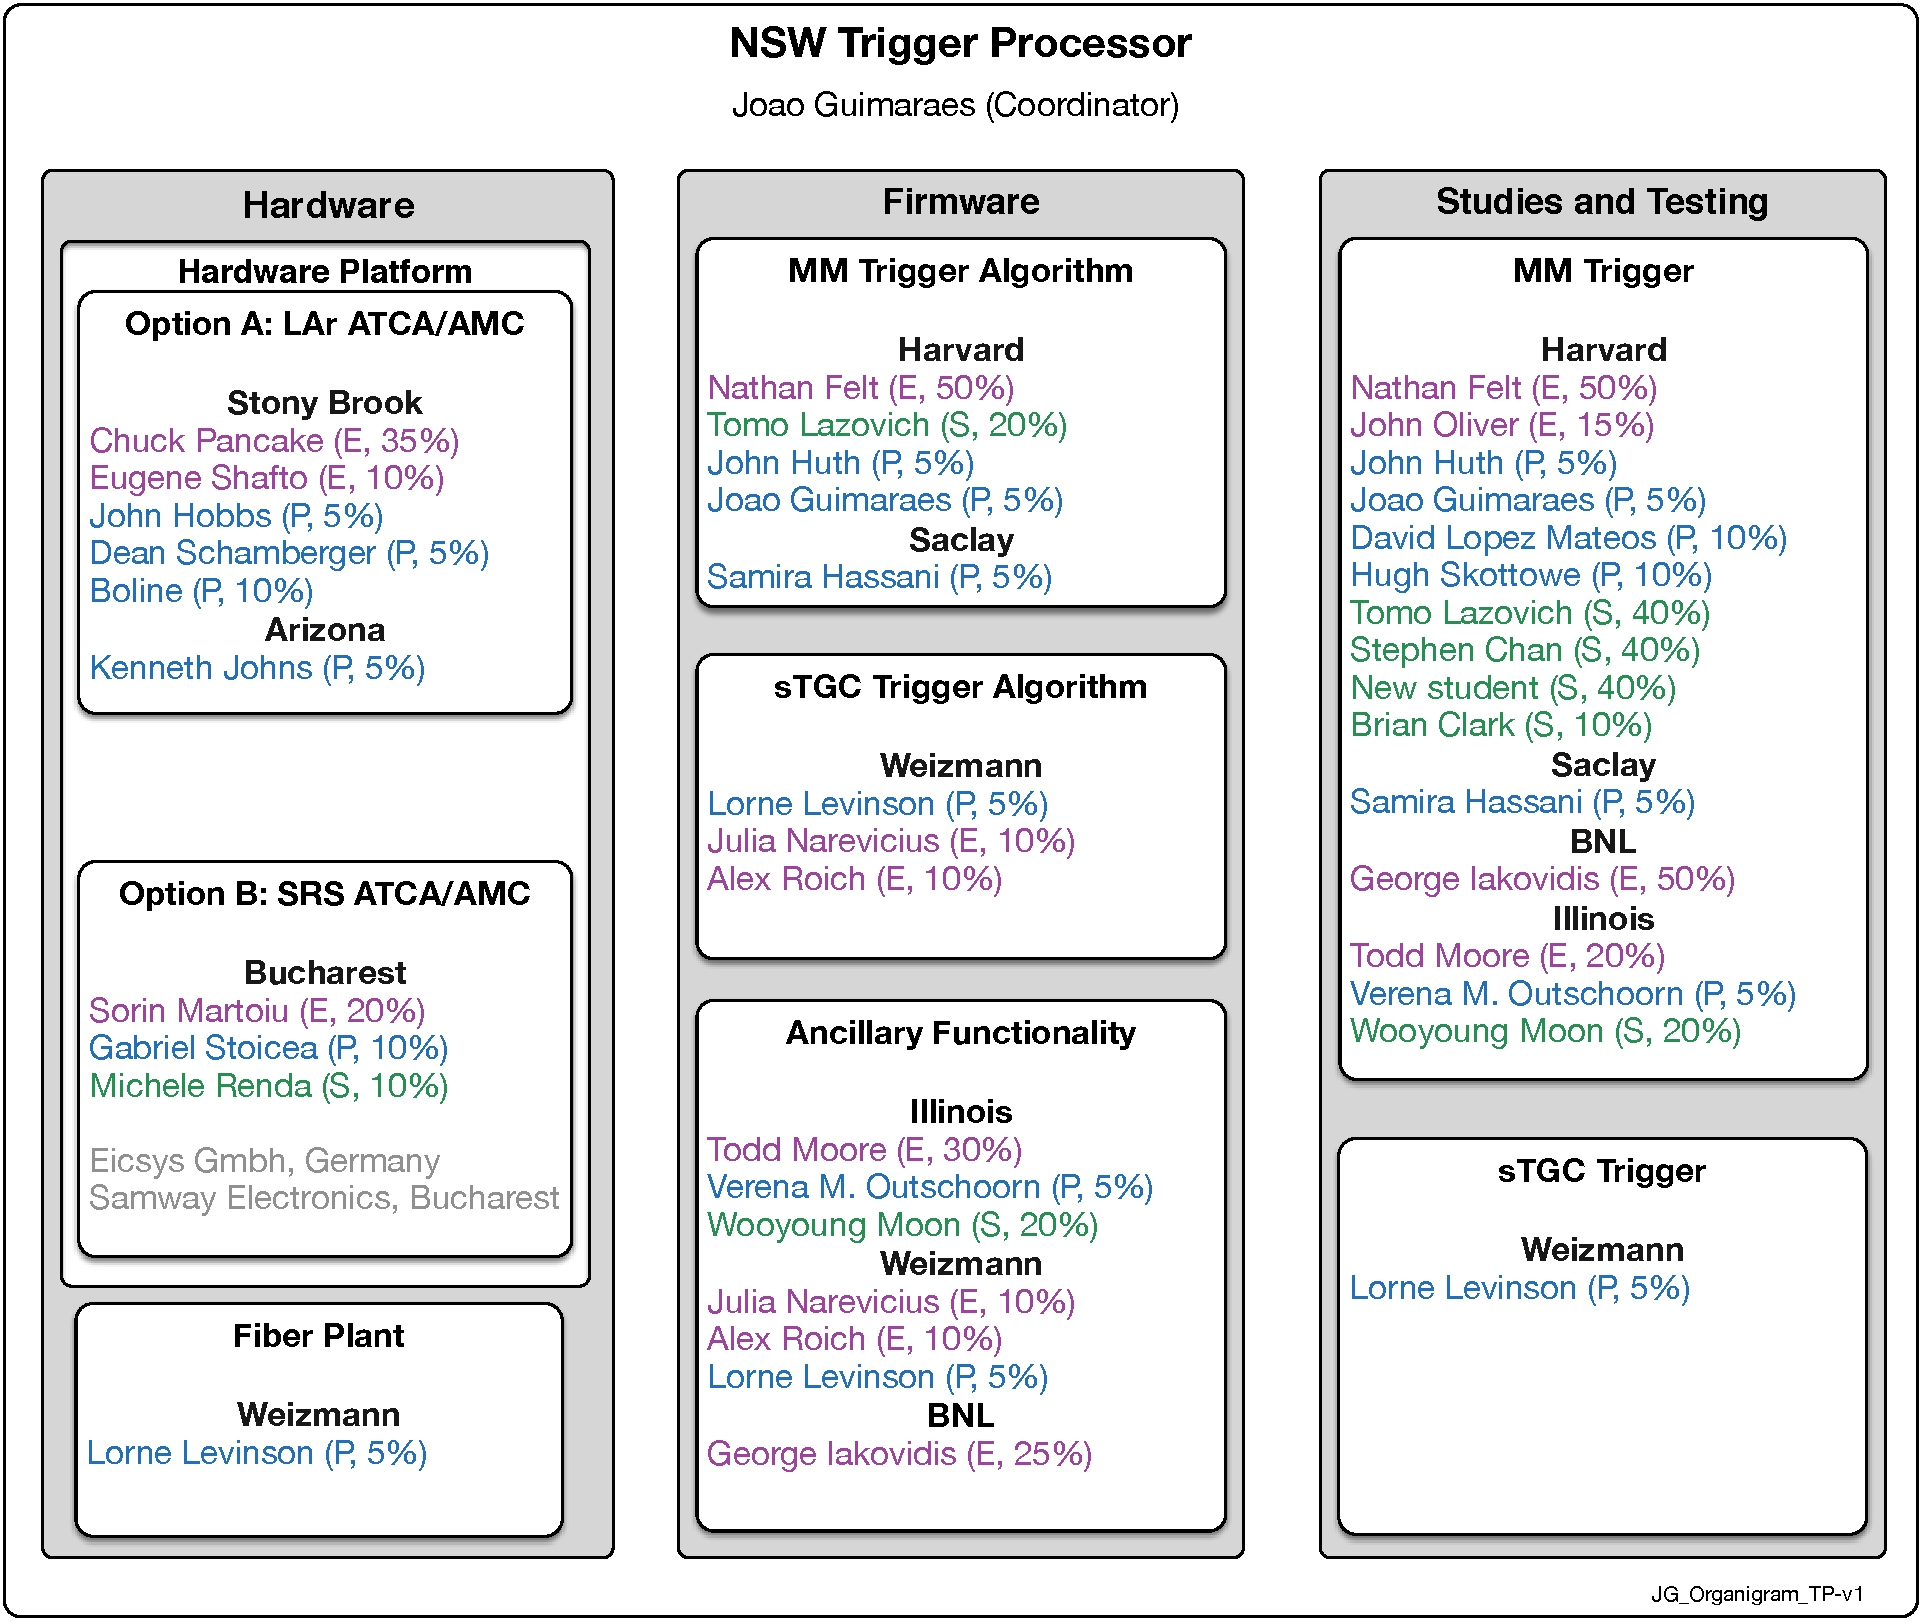
\includegraphics[width=0.95\textwidth]{figures/JG_Organigram_TP-v01.pdf}
        \caption{Organization and manpower dedicated to the Trigger Processor project, including engineers\,(E),  physicists\,(P) and students\,(S). The full-time equivalent estimations for each individual are also provided.}
        \label{fig:organigram}
    \end{center}
\end{figure}

\paragraph{Hardware}
\begin{description}
\item[LAr Hardware Platform] The LAr AMC-format Optical Test Card was designed by BNL, Stony Brook and Arizona for the LAr trigger upgrade. The card was not adopted by the LAr trigger project although prototypes exist and they are fully functional and tested. This card could fulfill the requirements of the TP but it requires updates to increase the bandwidth communication between mezzanine cards. The corresponding ATCA carrier board is designed and it will be used by the LAr trigger. It also requires updates to increase the inter-mezzanine bandwidth. Stony Brook and Arizona will design and implement the modifications required for the muon trigger project. Only this effort is indicated in Figure~\ref{fig:organigram}.
It includes 0.35 FTE enginnering for design updates to the boards and firmware, 0.1 FTE engineering for production hardware testing, 0.1\,FTE labor for production hardware testing and 0.1 FTE for technical oversight.

\item[SRS Hardware Platform] The ATCA-SRS carrier board was designed within the RD51 Collaboration and it is already available. An update is planned for mid-2015 but not deemed essential for this project. The ATCA-SRS Carrier Board is being manufactured under a licensing contract between Eicsys Gmbh, Germany licensee and the IP Holder Consortium within RD51 collaboration (CERN, IFIN-HH and Polytechnic University of Valencia), as licensor. The licensing contract is not exclusive.

The High-Density Optical Receiver (HORX) mezzanine board is a responsibility of IFIN-HH, Bucharest. Its design and realization is being done by an external specialized company (Samway Electronics, Bucharest). The final design is part of the contracted deliverables; therefore all design sources are in possession of IFIN-HH~\cite{hardware-SRS-Mezz}.

Apart from the two companies mentioned, which will provide support for the two boards, the following IFIN-HH team will be in charge of the design, specifications and firmware \& software support: Sorin Martoiu\,(0.2 FTE), Research Engineer; Michele Renday, Graduate Student\,(0.1\,FTE); and Gabriel Stoicea, Physicist\,(0.1\,FTE).


\item[Fiber plant] The Trigger Processor i/o fibers are integrated in the fiber plant (Appendix~\ref{app:specs-fibers}) that is the responsibility of the Weizmann Institute.
\end{description}

\paragraph{Firmware} includes algorithms and ancillary functionality firmware development. The bulk of the resources for firmware testing is included in the ``trigger studies and testing'' item.
\begin{description}
\item[MM Fitter Algorithm] The algorithm has been developed by the Harvard group. Previous contributions have been made by the postdoc and students listed under trigger studies in Figure~\ref{fig:organigram}. The same team will continue supporting the algorithm. Moving forward the algorithm firmware will be done by Nathan Felt (0.5\,FTE) with support from students and oversight from John Huth and Jo\~{a}o Guimar\~{a}es.
\item[MM Look-Up-Table Algorithm] The algorithm has been developed by the Saclay group, with contributions from Samira Hassani, Hevré le Provost, Claude Guyot and Philippe Schune. The team is being revamped and they are now focusing on the cavern background simulation. More contributions are expected in the longer term.
\item[sTGC Algorithm] The algorithm has been developed and will continue to be developed by the Weizmann group. The team includes Lorne Levinson and 0.2\,FTE of engineering support (Julia Narevicius and Alex Roich).
\item[Ancillary Functionality] Several groups have taken responsibility for delivering the firmware for the ancillary functions. These include Illinois, Weizmann and BNL. The Arizona group will also help, in particular if the LAr platform option is chosen, given that many of these functions are common to the LAr trigger board. The manpower pledged currently includes 0.75\,FTE engineering and 0.2\,FTE of student support. Lorne Levinson and Verena Outschoorn will oversee the project.
\end{description}


\paragraph{Trigger studies and testing} Most of the people currently making trigger studies will also be the manpower for future testing of the trigger hardware, firmware and performance. Given the different timescales both tasks are considered together.
\begin{description}
\item[MM Trigger] The trigger algorithm studies have been done by a small team of students and postdocs. Moving forward this team will be enlarged to include support for the trigger testing at home institutions and at CERN. Harvard, Saclay, BNL and Illinois are expected to contribute with a total of 1.35\,FTE engineering, 0.40\,FTE physicist and 1.5\,FTE student support.
\item[sTGC Trigger] The manpower pledged for the sTGC trigger studies and testing is limited to Lorne Levinson (0.05\,FTE). Although some of the hardware tests will be common with the ones from the MM trigger, this team needs to be enlarged.
\end{description}



\begin{comment}

Saclay: Future????

Saclay team who contributed to the trigger algorithm:
Samira Hassani
Hevré le Provost
Claude Guyot
Philippe Schune


\subsubsection{In the graph}

Stony brook:

Dean and I talked about the incremental manpower we'd need for the R&D  related changes to the AMC and ATCA carrier beyond the work already needed for LAr.   We estimate about 3 months of labor, roughly 1 month for the AMC and 2 months for the carrier.   We'll refine the estimate a bit this week to include incremental labor associated with production.  This will matter for the AMC more than the carrier.

As far as personnel availability goes, the engineer who has been doing the AMC card will basically finish that in the next month or so.   He would then be free to work on the mods for the AMC card.   Either he or Dean would do the layout changes for the carrier.

The original 0.25 FTEs is the engineering needed to make the AMC and carrier design changes to add four AMC ports to make a total of 16 LVDS connections available(primarily layout updates).  We've also now estimated the additional FTEs for testing firmware changes and production testing.  The full list is

0.25 FTE engineering (Chuck Pancake) for design  updates to AMC and carrier
0.1   FTE engineering for updates to LVDS testing firmware (Pancake)
0.1   FTE engineering for production hardware testing (Eugene Shafto)
0.1   FTE off project labor for production hardware testing (post doc, Boline; students)
0.1   FTE off project technical oversight Schamberger/Hobbs



Illinois:
Todd 30\% firmware, 20% testing
Wooyoung 20\% firmware, 20% testing
Verena 5\% firmware, 5% testing, 40% software (I’m not teaching the summer & fall)

Todd Moore
Research Engineer
ancillary functions
testing, including hardware

Wooyoung Moon
Graduate student
firmware development and testing
commissioning, including integration at cern


Weizmann:
Julia Narevicius, Alex Roich, Lorne Levinson (Algorithm development and corresponding firmware implementation, Ancillary functions firmware)
Julia and Alex are each 20\% on NSW TP (and another 20% each on FELIX).

Bucharest:
The following team from our institute will be in charge of the design, specifications and firmware & software support,
Sorin Martoiu, Research Engineer, 20\%
Michele Renda, Graduate Student, 10\%
Gabriel Stoicea, Physicist, 10\%

BNL:
Brookhaven will soon have an Electronic Engineer full time Ph.D. (George Iakovidis) working on
the firmware ancillary TP tasks, test beams and analysis, CERN vertical slice coordination and, eventually, commissioning.

Harvard:
John Huth 15\%
Joao
Nathan 100\% (50/50)
John Oliver 15\% - testing
Possible new student


\paragraph{Hardware platform}
\vspace{-5mm}
\begin{itemize}\itemsep-4pt
        \vspace{-1mm}
	\item LAr Card (option A):
	\begin{itemize}\itemsep-6pt
	    \vspace{-2mm}
	    \item Arizona (\emph{Kenneth Johns})
	    \item BNL
	    \item Stony Brook (John Hobbs)
	\end{itemize}\itemsep-4pt
	\item SRS Card (option B):
	\begin{itemize}\itemsep-4pt\parskip-4pt\parsep-4pt
	    \vspace{-1mm}
	    \item Bucharest (Sorin Martoiu)
	\end{itemize}
\end{itemize}

\paragraph{Algorithm development and corresponding firmware implementation}
\vspace{-5mm}
\begin{itemize}\itemsep-6pt
	\item Harvard
	\item Saclay
	\item Weizmann (Julia Narevicius, Alex Roich, Lorne Levinson)
\end{itemize}

\paragraph{Ancillary functions firmware}
\vspace{-5mm}
\begin{itemize}\itemsep-6pt
	\item Arizona (Ken Johns)
	\item Harvard
	\item Illinois (Verena Martinez Outschoorn, Todd Moore, )
	\item Weizmann (Julia Narevicius, Alex Roich, Lorne Levinson)
\end{itemize}

\paragraph{Testing}
\vspace{-5mm}
\begin{itemize}\itemsep-6pt
	\item Harvard (Tomo Lazovich, Hugh Skottowe, Nathan Felt)
	\item Illinois
	\item Weizmann
\end{itemize}

\paragraph{Software}
\begin{itemize}
	\item Michigan...
\end{itemize}

\end{comment}

